\newpage % Rozdziały zaczynamy od nowej strony.
\section{Analiza skuteczności algorytmów}

\subsection{Metody testowania}
\indent\ Testy zostały przeprowadzone za pomocą testów jednostkowych, w których wszystkie algorytmy zostały zestawione przeciwko sobie. Statki były rozstawione losowo dla obu stron. Wszystkie testy jednostkowe dziedziczą po klasie bazowej AlgorithmTestBase, która była potrzebna do inicjalizacji lub zmockowania wszelkich potrzebnych serwisów. Na listingu 12 widoczny jest przykładowy test jednostkowy. Testowane były oba warianty zasady stykania się statków. Stała numberOfIterations wynosiła 1000, więc dla każdego zestawienia algorytmów i zasad otrzymano 1000 wyników. Ogólnie podczas testów zebrano około 40 000 rekordów w kontenerze TestGameSessions.

\begin{addmargin}[10mm]{0mm}
\begin{lstlisting}[
    language={[Sharp]C},
    numbers=left,
    firstnumber=11,
    caption={Przykładowy test jednostkowy},
    aboveskip=0pt
]
[Fact]
public void VsRandomShipsCantTouch()
{
    _httpContextAccessor.SetupTestHttpContext();

    var initialGameState = new GameState
    {
        PlayerAiType = AiType.LocationHeuristic,
        OpponentAiType = AiType.Random,
        ShipsCanTouch = false,
    };

    var playerWins = TestHelper.RunSimulation(
        initialGameState,
        _gameStateService,
        _generateMoveService,
        _shipLocationService,
        numberOfIterations);

    Assert.True(true);
}
\end{lstlisting}
\end{addmargin}


\subsection{Wyniki testów algorytmów}
W tabelach widocznych w poniższych rozdziałach stosowane będą skrócone nazwy algorytmów, tak aby bez problemu mieściły się w komórkach tabel. Poniżej znajduje się objaśnienie skrótów.
\begin{itemize}
    \item \textbf{Max. zysk} - Algorytm oparty na heurystyce maksymalizacji zysku ze strzału.
    \item \textbf{Analiza trafień} - Algorytm oparty na heurystyce najbardziej prawdopodobnej lokalizacji na podstawie trafień.
    \item \textbf{Max. zysk rozszerzony} - Algorytm oparty na heurystyce maksymalizacji zysku priorytetyzującej dłuższe statki.
    \item \textbf{Max. zysk + analiza trafień} - Algorytm oparty na heurystykach maksymalizacji zysku oraz najbardziej prawdopodobnej lokalizacji na podstawie trafień.
    \item \textbf{Max. zysk rozszerzony + analiza trafień} - Algorytm oparty na heurystykach maksymalizacji zysku oraz najbardziej prawdopodobnej lokalizacji na podstawie trafień priorytetyzującej dłuższe statki. 
\end{itemize}

W tabelach przedstawiających skuteczność poszczególnych algorytmów posłużono się kolorami, w celu podkreślenia otrzymanych wartości:
\begin{itemize}
    \item Kolor zielony - wynik zdecydowanie lepszy, skuteczność powyżej 55\%
    \item Kolor żółty - wynik porównywalny, skuteczność pomiędzy 45\%-55\%
    \item Kolor czerwony - wynik zdecydowanie gorszy, skuteczność poniżej 45\%
\end{itemize}

\subsubsection{Algorytm losowy}

Algorytm losowy, zgodnie z przewidywaniami wypadł najgorzej w zestawieniu z innymi algorytmami. W tabeli 6.1 widać, że najwyższy procent zwycięstw jaki osiągnął to 13,1\% przeciwko algorytmowi losowemu rozszerzonemu. Wśród wyników można zaobserwować prawidłowość, że skuteczność delikatnie wzrasta w przypadku testów, gdzie statki mogą się stykać. Zgodnie z tym co zostało wspomniane pod koniec rozdziału 2.2, dodatkowe ograniczenie tego, jak mogą być rozstawione statki, ułatwia heurystykom analizę planszy przeciwnika. Gdy tego ograniczenia nie ma, gra staje się trochę bardziej losowa - chociaż nadal algorytmy oparte na heurystykach są znacznie skuteczniejsze od algorytmu losowego.

\begin{table}[!h]
    \centering
    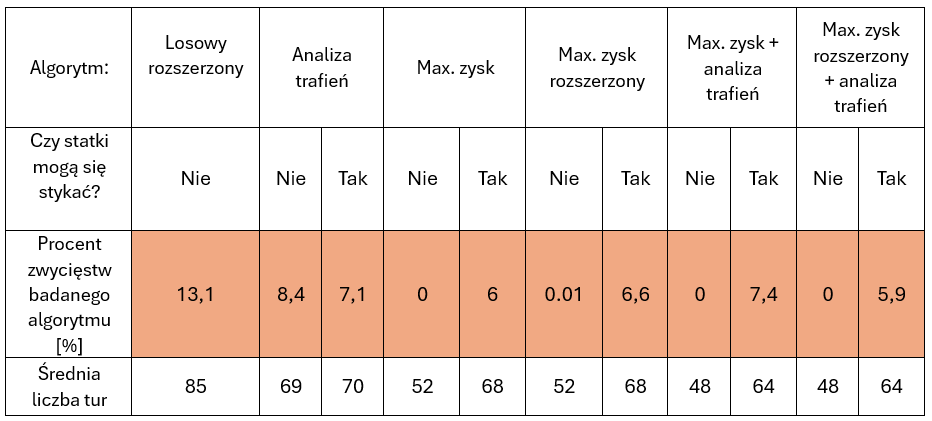
\includegraphics[width=1\linewidth]{img/table-random.png}
    \caption{Wyniki testów dla algorytmu losowego}
\end{table}

\subsubsection{Algorytm losowy z pominięciem pól sąsiadujących z zatopionymi statkami}

Algorytm losowy z pominięciem pól był testowany jedynie w przypadku gdy statki nie mogą się ze sobą stykać. W przeciwnym wypadku, gdyby oponent ustawił statki obok siebie, badany algorytm nie byłby w stanie odnieść zwycięstwa. W wynikach testów widocznych w tabeli 6.2 widać, że algorytm rozszerzony jest dużo skuteczniejszy od swojej podstawowej wersji. Można też zauważyć zdecydowany wzrost skuteczności przeciwko algorytmowi opartemu na heurystyce najbardziej prawdopodobnej lokalizacji na podstawie trafień. W pozostałych przypadkach również można zaobserwować wzrost skuteczności, ale jest on bardzo niewielki.
Test

\begin{table}[!h]
    \centering
    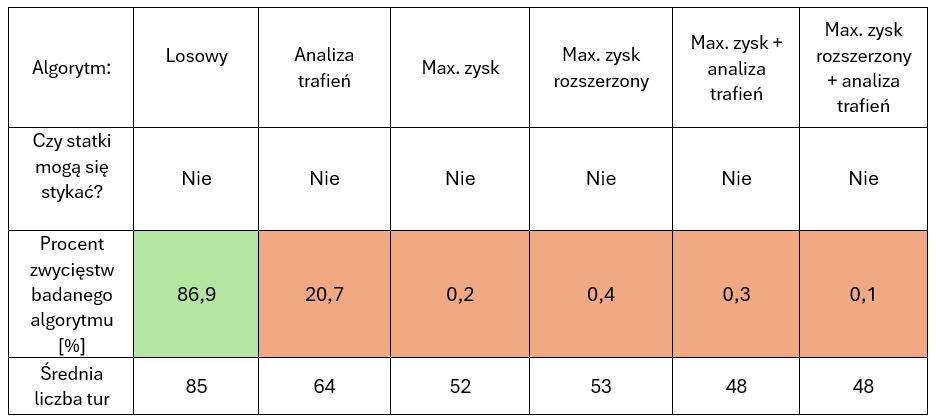
\includegraphics[width=1\linewidth]{img/table-random-plus.png}
    \caption{Wyniki testów dla algorytmu losowego rozszerzonego}
\end{table}

\subsubsection{Algorytm oparty na heurystyce najbardziej prawdopodobnej lokalizacji na podstawie trafień}

Jak widać w tabeli 6.3, w przypadku tego algorytmu widać wyraźnie jego przewagę nad algorytmami losowymi. Jest on jednak zdecydowanie najsłabszym z algorytmów heurystyczych. Umiejętność 'dobijania' trafionych statków wyróżnia go na tle algorytmów losowych, ale nadal jednak w dużej mierze opiera się na losowości - jeśli na planszy przeciwnika nie ma żadnego trafienia, algorytm oddaje strzały w losowe komórki.

Podobnie jak w 6.2.1, widać znaczące różnicę w zależności od wyboru zasad - skuteczność tego algorytmu wzrasta gdy statki mogą się ze sobą stykać.

\begin{table}[!h]
    \centering
    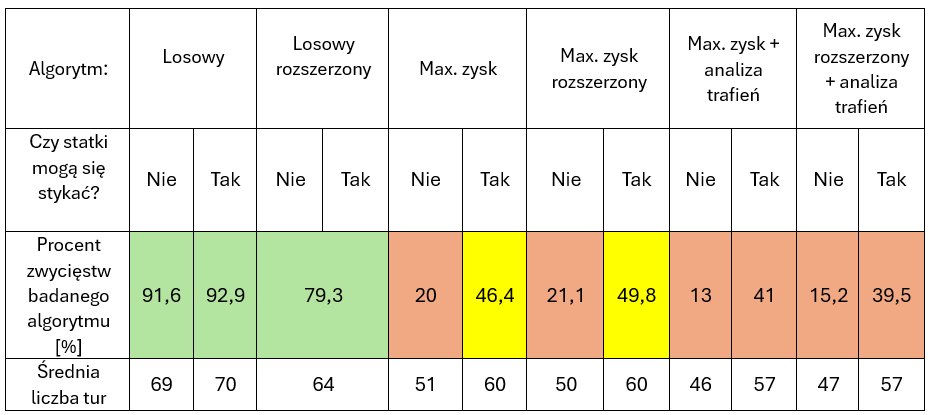
\includegraphics[width=1\linewidth]{img/table-hit-heuristic.png}
    \caption{Wyniki testów dla algorytmu opartego na heurystyce najbardziej prawdopodobnej lokalizacji na podstawie trafień}
\end{table}

\subsubsection{Algorytm oparty na heurystyce maksymalizacji zysku ze strzału}

Widać tu wzrost skuteczności o około 10\% względem względem algorytmów losowych. Algorytm jest też zdecydowanie skuteczniejszy od algorytmu opartego na heurystyce najbardziej prawdopodobnej lokalizacji na podstawie trafień, aczkolwiek gdy statki mogą się ze sobą stykać to ich skuteczność jest porównywalna.

\begin{table}[!h]
    \centering
    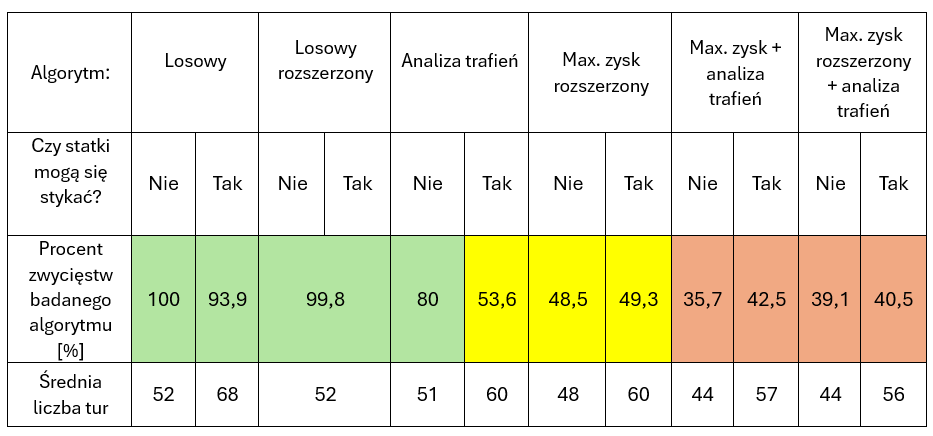
\includegraphics[width=1\linewidth]{img/table-location-heuristic.png}
    \caption{Wyniki testów dla algorytmu opartego na heurystyce maksymalizacji zysku ze strzału}
\end{table}


\subsubsection{Algorytm oparty na heurystyce maksymalizacji zysku priorytetyzującej dłuższe statki}

Wyniki są widoczne w tabeli 6.5 i są bardzo zbliżone do wartości z punktu 6.2.4. Można zaobserwować, że w bezpośrednim starciu, badany algorytm jest nieznacznie skuteczniejszy od swojego podstawowego wariantu. Jednak we wszystkich pozostałych przypadkach poza jednym widoczny jest nieznaczny spadek skuteczności, w najgorszym przypadku 3,5\%.

\begin{table}[!h]
    \centering
    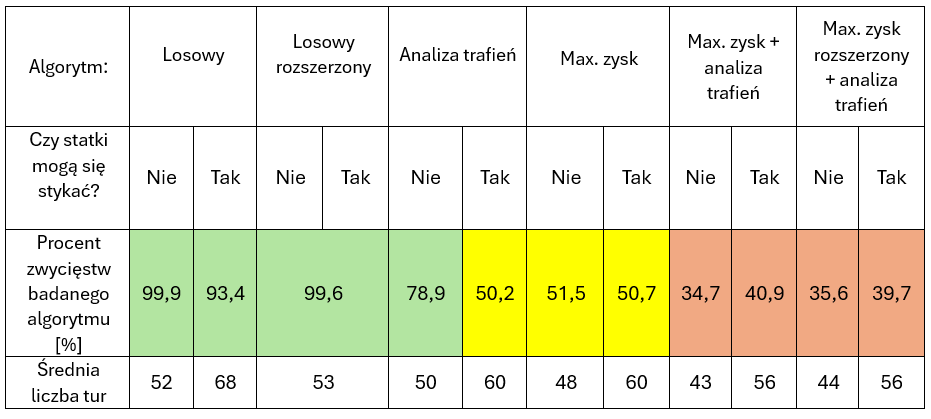
\includegraphics[width=1\linewidth]{img/table-location-heuristic-extended.png}
    \caption{Wyniki testów dla algorytmu opartego na heurystyce maksymalizacji zysku priorytetyzującej dłuższe statki}
\end{table}

\subsubsection{Algorytm oparty na heurystykach maksymalizacji zysku oraz najbardziej prawdopodobnej lokalizacji na podstawie trafień}

Jak widać na tabeli 6.6, algorytm wygrywa w zestawieniu ze wszystkimi pozostałymi algorytmami, poza swoją rozszerzoną wersją. Największy wzrost skuteczności widać przeciwko algorytmom \emph{Analiza trafień} oraz \emph{Max.zysk}. Wynika to z faktu, że badany algorytm jest usprawnieniem \emph{Max.zysk} poprzez umożliwienie algorytmowi 'dobijania' trafionych statków.

\begin{table}[!h]
    \centering
    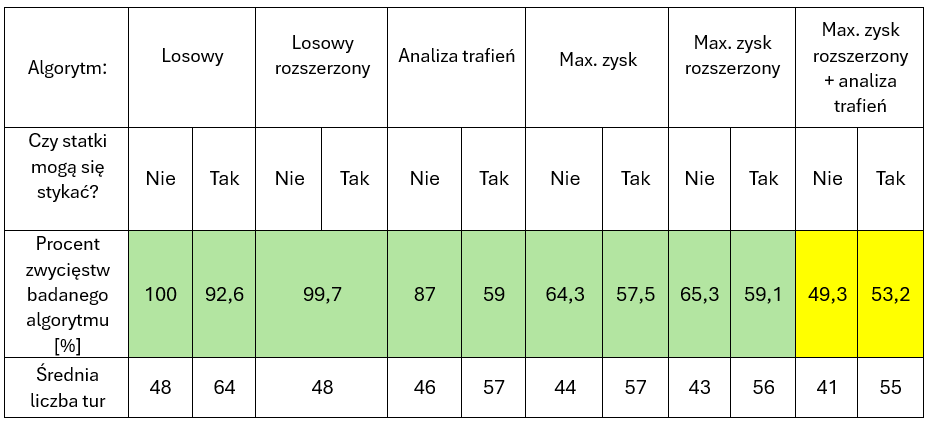
\includegraphics[width=1\linewidth]{img/table-location-hit-heuristic.png}
    \caption{Wyniki testów dla algorytmu opartego na heurystykach maksymalizacji zysku oraz najbardziej prawdopodobnej lokalizacji na podstawie trafień}
\end{table}

\subsubsection{Algorytm oparty na heurystykach maksymalizacji zysku oraz najbardziej prawdopodobnej lokalizacji na podstawie trafień priorytetyzującej dłuższe statki}

Podobnie jak w przypadku 6.2.5, wyniki wersji podstawowej i rozszerzonej algorytmu są bardzo zbliżone. W bezpośrednich starciu wersja rozszerzona jest nieznacznie skuteczniejsza gdy statki nie mogą się ze sobą stykać. W przeciwnym wypadku, lepiej wypada wersja podstawowa algorytmu. W starciach z pozostałymi algorytmami wyniki są zbliżone.

\begin{table}[!h]
    \centering
    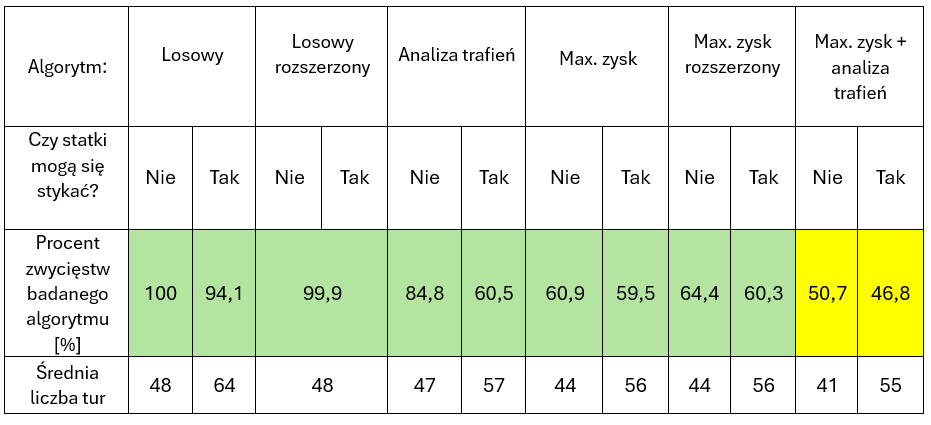
\includegraphics[width=1\linewidth]{img/table-location-extended-hit-heuristic.png}
    \caption{Wyniki testów dla algorytmu opartego na heurystykach maksymalizacji zysku oraz najbardziej prawdopodobnej lokalizacji na podstawie trafień priorytetyzującej dłuższe statki}
\end{table}

\subsection{Podsumowanie}

Aby wyłonić najskuteczniejszy algorytm, stworzone zostały tabele 6.8 oraz 6.9. Przedstawiają one zestawienie pojedynków pomiędzy wszystkimi algorytmami. Tabela 6.8 przedstawia wyniki, gdy statki nie mogą się ze sobą stykać, a tabela 6.9. przeciwny przypadek. W każdej kolumnie na zielono zaznaczone zostały komórki zawierające najwyższą skuteczność. Oznacza to, że algorytm przypisany do danego wiersza, był najskuteczniejszy w starciu z algorytmem przypisanym do danej kolumny.

Korzystając z tych tabelę, można zaobserwować:

\begin{itemize}
    \item Gdy statki nie mogą się ze sobą stykać, podstawowa wersja  \emph{Max. zysk + analiza trafień} jest najskuteczniejsza w prawie wszystkich przypadkach. 
    \item Gdy statki mogą się ze sobą stykać, rozszerzona wersja  \emph{Max. zysk + analiza trafień} jest najskuteczniejsza w prawie wszystkich przypadkach, poza bezpośrednim starciem ze swoją podstawową wersją.
\end{itemize}

Widać więc wyraźnie wpływ różnicy zasad na wyniki. Ciekawe jest to, że w obu przypadkach ogólnie najskuteczniejszy algorytm przegrywał w starciu ze swoim drugim wariantem.

Aby ostatecznie rozstrzygnąć, który algorytm jest skuteczniejszy spróbowano również policzyć ich ogólną skuteczność. Dokonano tego poprzez obliczenie średniej ze skuteczności przeciwko poszczególnym algorytmom. Przekłada się to na następujące wyniki procentowe:

\begin{itemize}
    \item 70,94\% dla wersji podstawowej
    \item 70,51\% dla wersji rozszerzonej
\end{itemize}

Nieznacznie skuteczniejszy jest więc wersja podstawowa \emph{Max. zysk + analiza trafień}.
\begin{table}[!h]
    \centering
    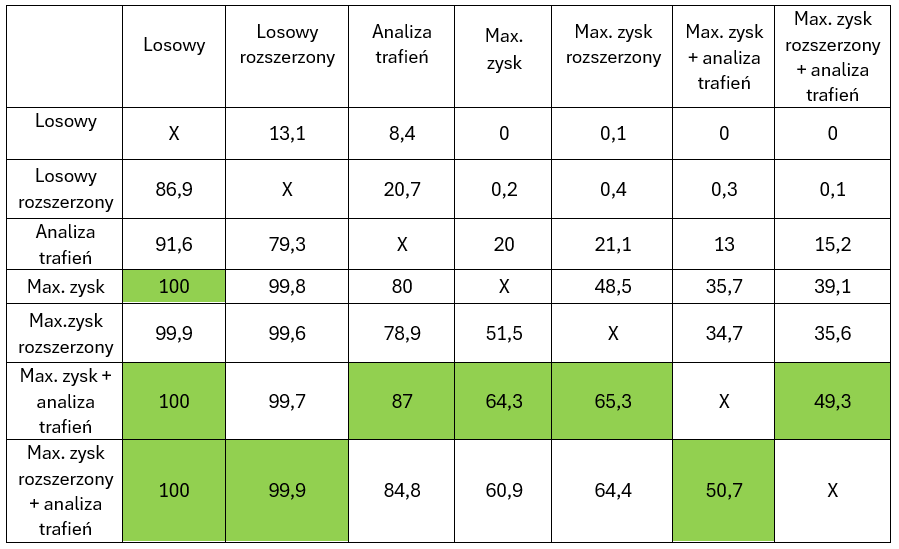
\includegraphics[width=1\linewidth]{img/summary-ships-cant-touch.PNG}
    \caption{Podsumowanie testów gdy statki nie mogą się ze sobą stykać}
\end{table}

\begin{table}[!h]
    \centering
    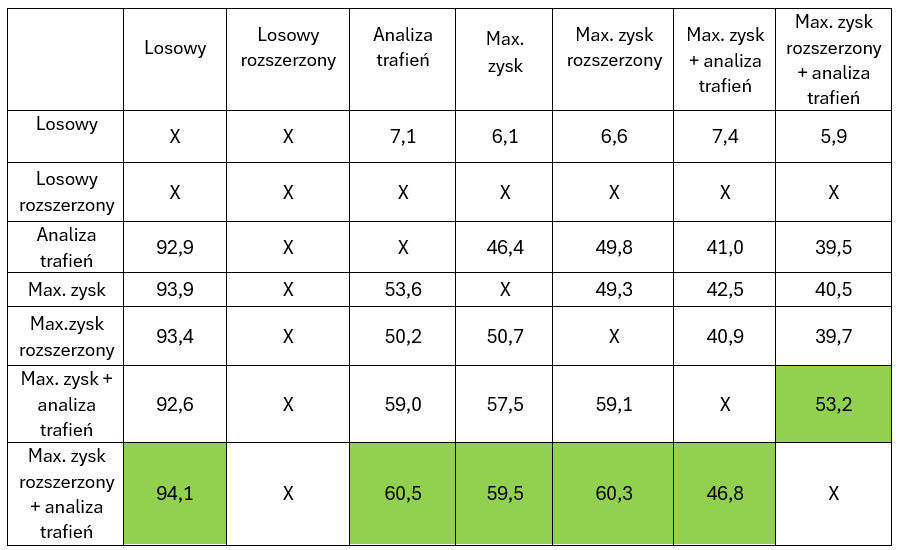
\includegraphics[width=1\linewidth]{img/summary-ships-can-touch.PNG}
    \caption{Podsumowanie testów gdy statki mogą się ze sobą stykać}
\end{table}

Analogicznie obliczono zagregowane skuteczności dla wszystkich algorytmów, co przedstawia tabela 6.10. Przy obliczeniach wykorzystano zapytanie widoczne na listingu 13.

\begin{table}[!h]
    \centering
    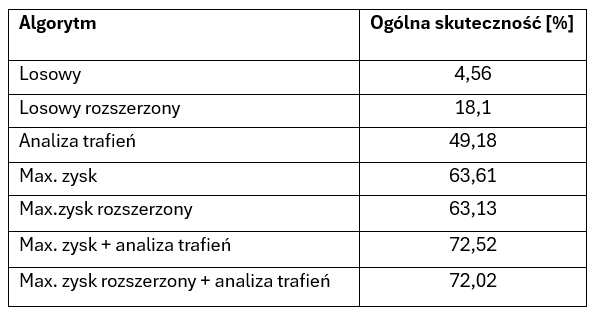
\includegraphics[width=0.7\linewidth]{img/aggregate.PNG}
    \caption{Zagregowane średnie skuteczności poszczególnych algorytmów}
\end{table}

\begin{addmargin}[10mm]{0mm}
\begin{lstlisting}[
    language=SQL,
    numbers=left,
    firstnumber=1,
    caption={Zapytanie do Azure Cosmos DB, w celu uzyskania zagregowanej skuteczności algorytmu},
    aboveskip=0pt
]
SELECT 
    AVG(
        IIF(c.playerMovesCount > c.opponentMovesCount,
        c.playerMovesCount,
        c.opponentMovesCount)
    ) AS avgMaxMoves
FROM c
WHERE (c.playerAiType = {ALG_1} AND c.opponentAiType = {ALG_2}
OR c.playerAiType = {ALG_2} AND c.opponentAiType = {ALG_1})
and c.shipsCanTouch = {WYBRANE_ZASADY}
\end{lstlisting}
\end{addmargin}

Na podstawie wyników stworzono wykres widoczny na rysunku 6.1. Algorytmy zostały posortowane od najmniej do najbardziej skutecznego.

\begin{figure}[!h]
    \label{fig:aggregate-chart}
    \centering 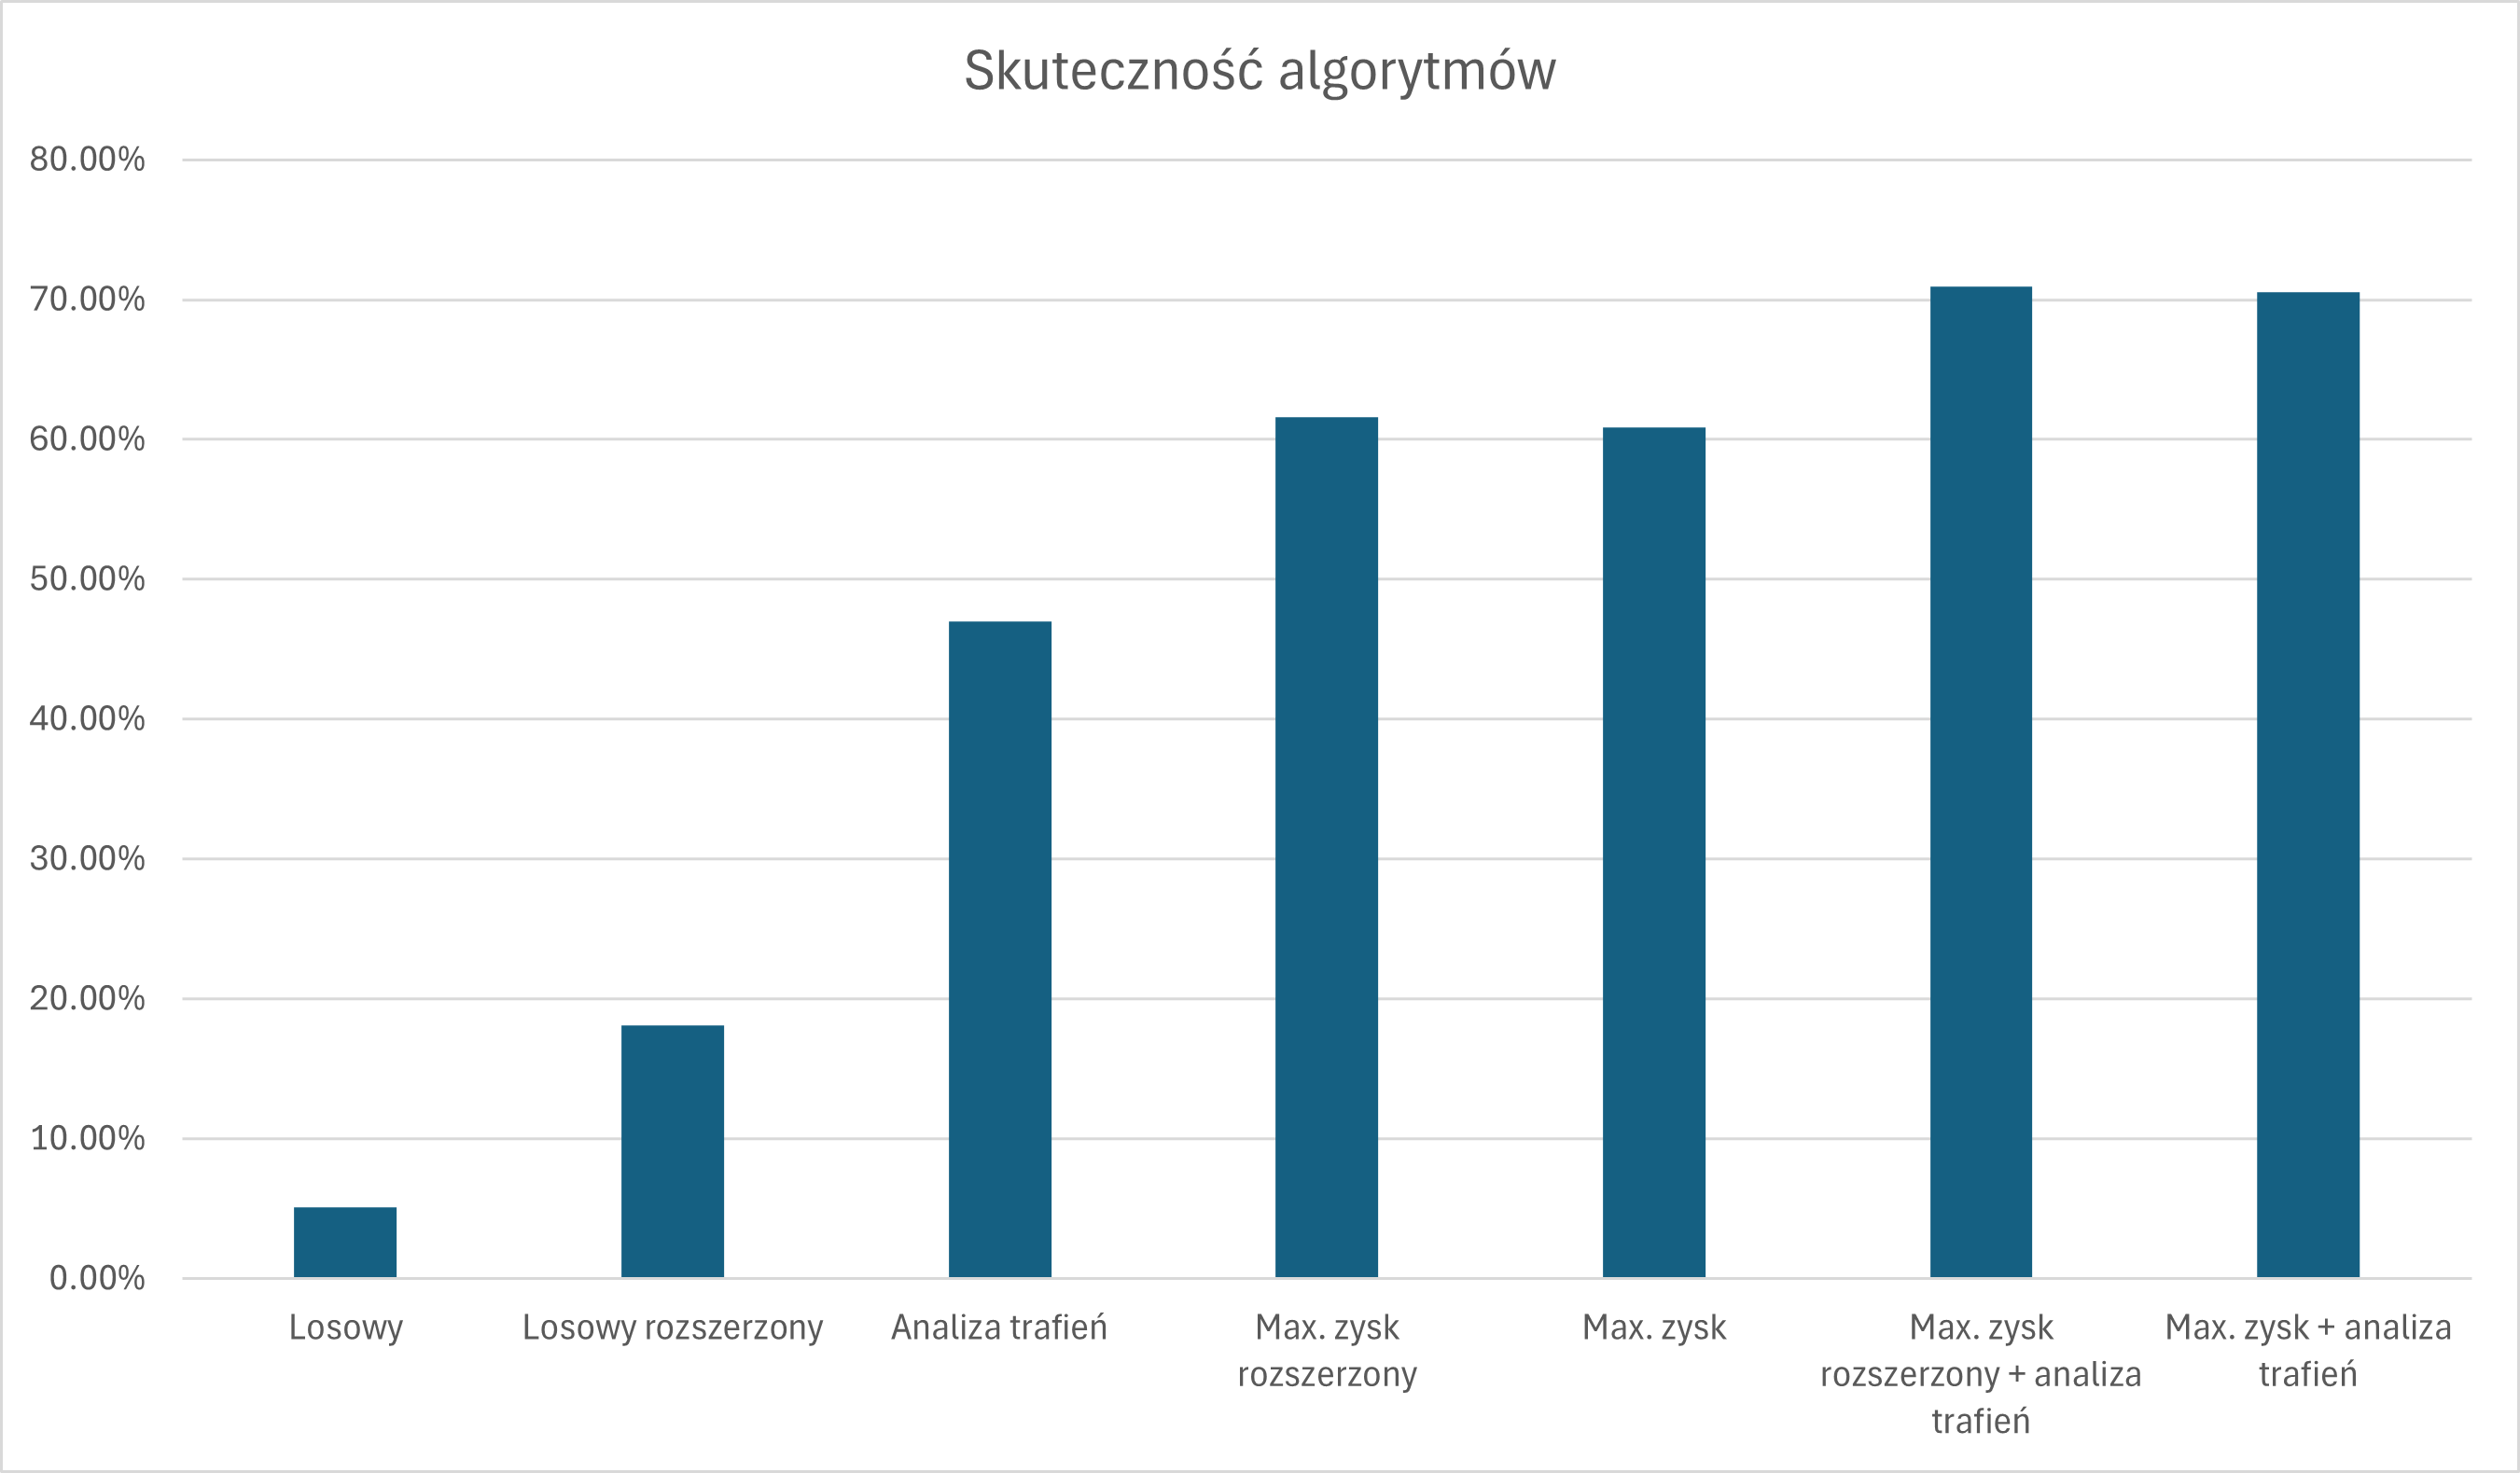
\includegraphics[width=0.9\linewidth]{img/aggregate-chart.png}
    \caption{Wykres zagregowanych średnich dla poszczególnych algorytmów.}
\end{figure}

Utworzono również wykres 6.2 ukazujący skuteczności różnych algorytmów w starciach z algorytmem losowym, aby lepiej zobrazować różnice w skuteczności zależnie od tego czy statki mogą się ze sobą stykać.

\begin{figure}[!h]
    \label{fig:round-avg}
    \centering 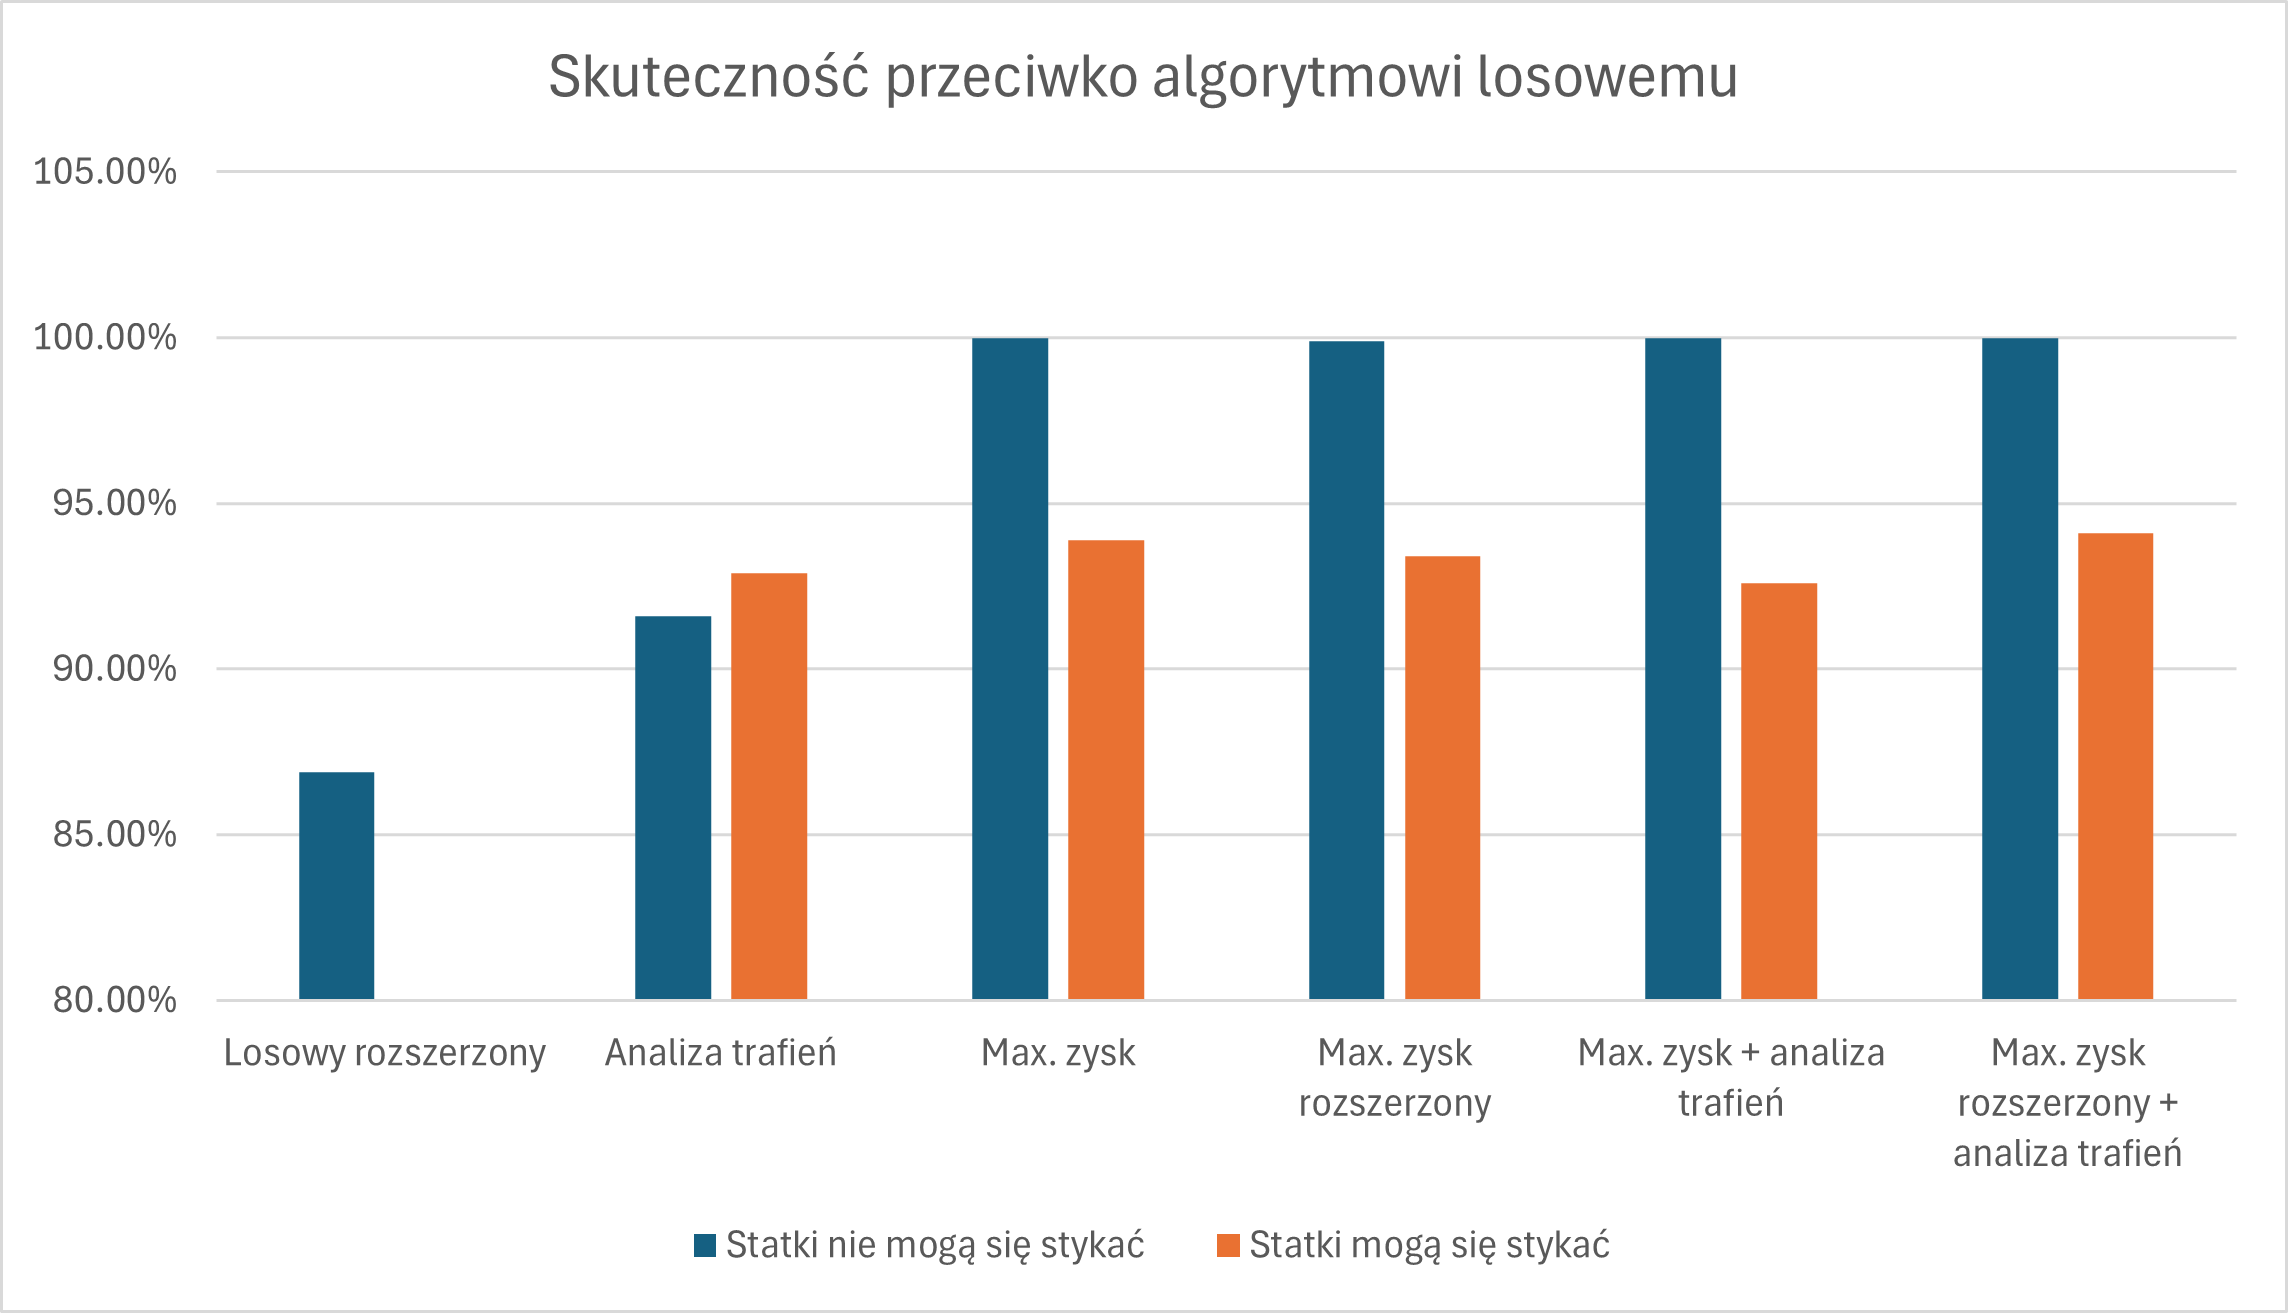
\includegraphics[width=0.9\linewidth]{img/chart-random-scores.png}
    \caption{Skuteczność algorytmów w starciach z algorytmem losowym.}
\end{figure}

Dla wszystkich zestawień algorytmów obliczono również średnią liczbę zagranych tur, zanim jedna ze stron odniosła zwycięstwo. Dane te widoczne są w tabelach 6.1-6.9 oraz na wykresie z rysunku 6.3, gdzie jako punkt odniesienia wykorzystano algorytm losowy.

\begin{figure}[!h]
    \label{fig:round-avg}
    \centering 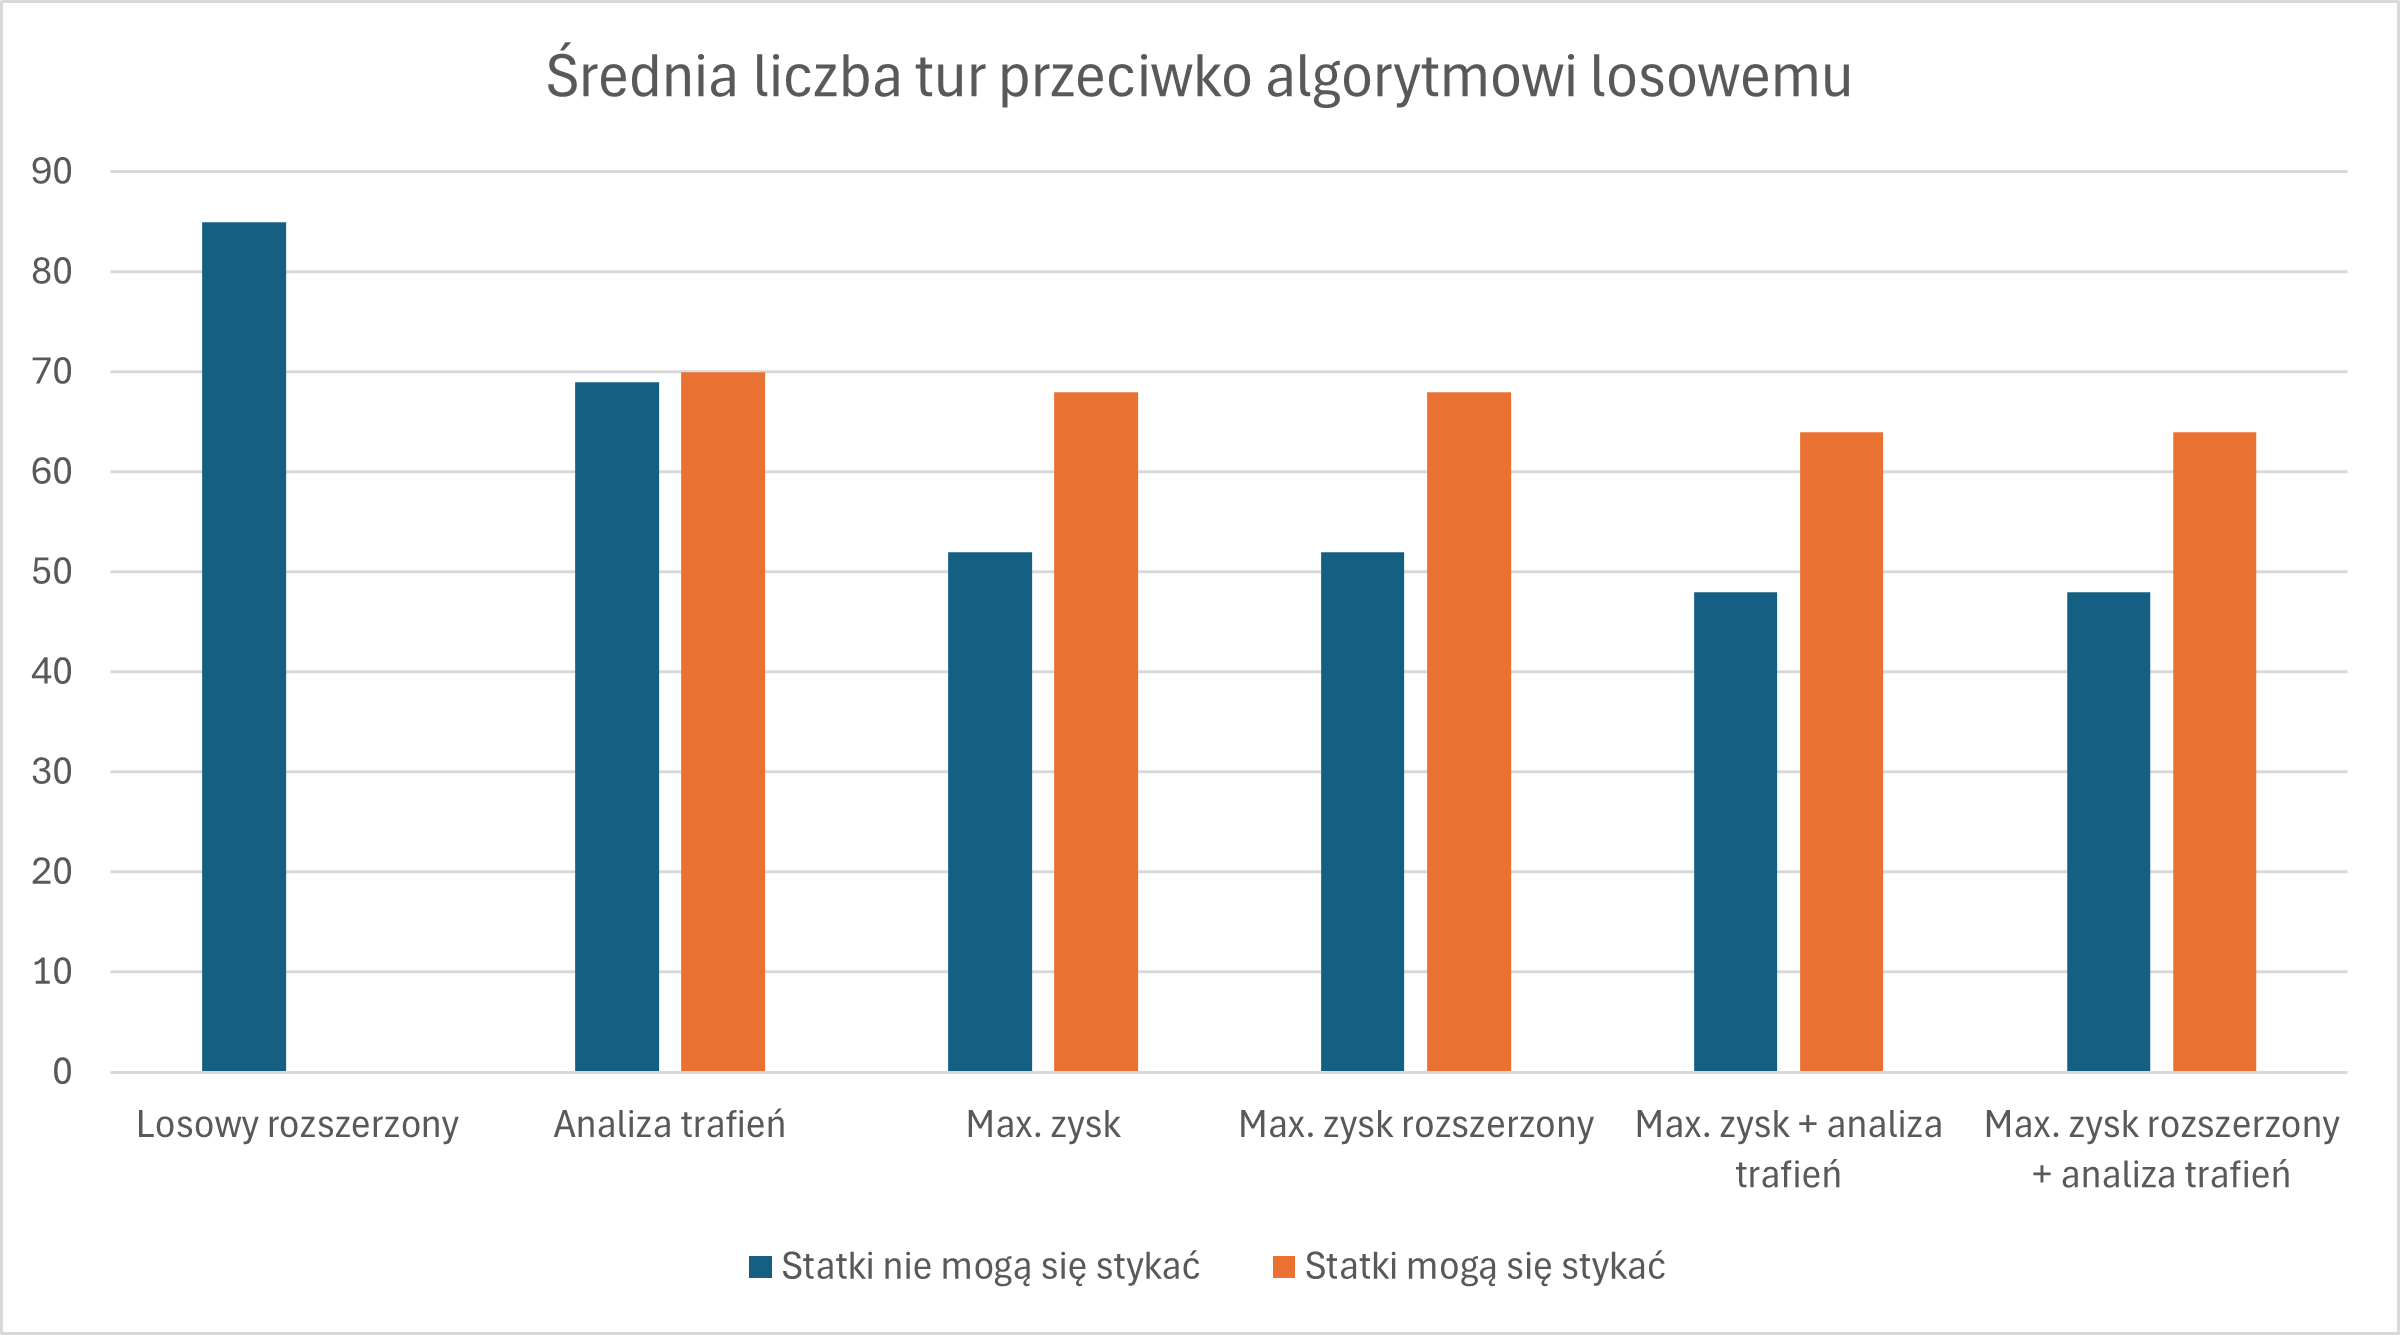
\includegraphics[width=0.9\linewidth]{img/round-count-avg.png}
    \caption{Średnia liczba tur w starciach z algorytmem losowym.}
\end{figure}


\subsection{Analiza rozgrywek z ludźmi}

Niestety nie udało się zebrać wystarczająco dużo danych, aby przeprowadzić dokładną analizę skuteczności algorytmów decyzyjnych przeciwko ludziom. Testy algorytm-algorytm opierały się na 1000 rozgrywek pomiędzy parami algorytmów, dla obu wariantów zasad. W przypadku testów z ludźmi, do analizy potrzebny byłoby 13 000 rozgrywek, ponieważ zaimplementowano 7 algorytmów, w tym jeden który dostępny jest jedynie gdy statki nie mogą się ze sobą stykać. Udało się zebrać dane dotyczące jedynie około 100 rozgrywek, a więc jedynie 1\% potrzebnej liczby. Przeprowadzona na ich podstawie analiza nie jest więc zbyt miarodajna, może być potraktowana raczej jako ciekawostka.

Większość użytkowników preferowała wybór zasad niepozwalających statkom się stykać - dlatego tylko ten przypadek będzie analizowany.

Na tabeli 6.11 oraz obrazującym ją wykresie z rysunku 6.12 widać, że ogólna tendencja skuteczności algorytmów jest podobna. Widać jej stopniowy wzrost, oraz spadek średniej liczby tur potrzebnej do pokonania gracza. Anomalią jest znaczny wzrost skuteczności w przypadku algorytmu \emph{Max. zysk}, ale wynika to najprawdopodobniej z małej próby badawczej. Dodatkowym czynnikiem utrudniającym miarodajną analizę wyników starć algorytm-gracz, jest fakt że nie każdy gracz gra na takim samym poziomie. Teoretycznie słabszy algorytm może mieć zawyżoną skuteczność, jeśli grało z nim  więcej 'słabszych' graczy. Dlatego konieczna jest większa ilość rozgrywek, aby wyeliminować wpływ tych czynników na ogół danych.

\begin{table}[!h]
    \label{fig:vs-people}
    \centering 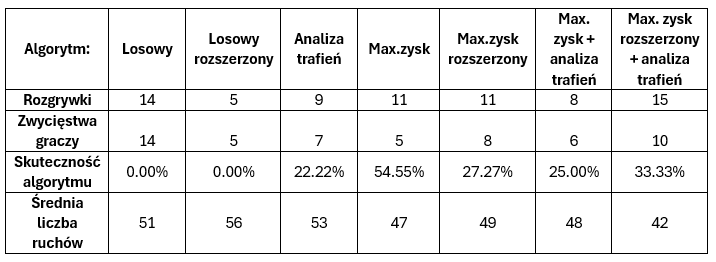
\includegraphics[width=0.9\linewidth]{img/vs_people.PNG}
    \caption{Skuteczność oraz średnia liczba ruchów algorytmów w starciach z graczami.}
\end{table}

\begin{table}[!h]
    \label{fig:vs-people-chart}
    \centering 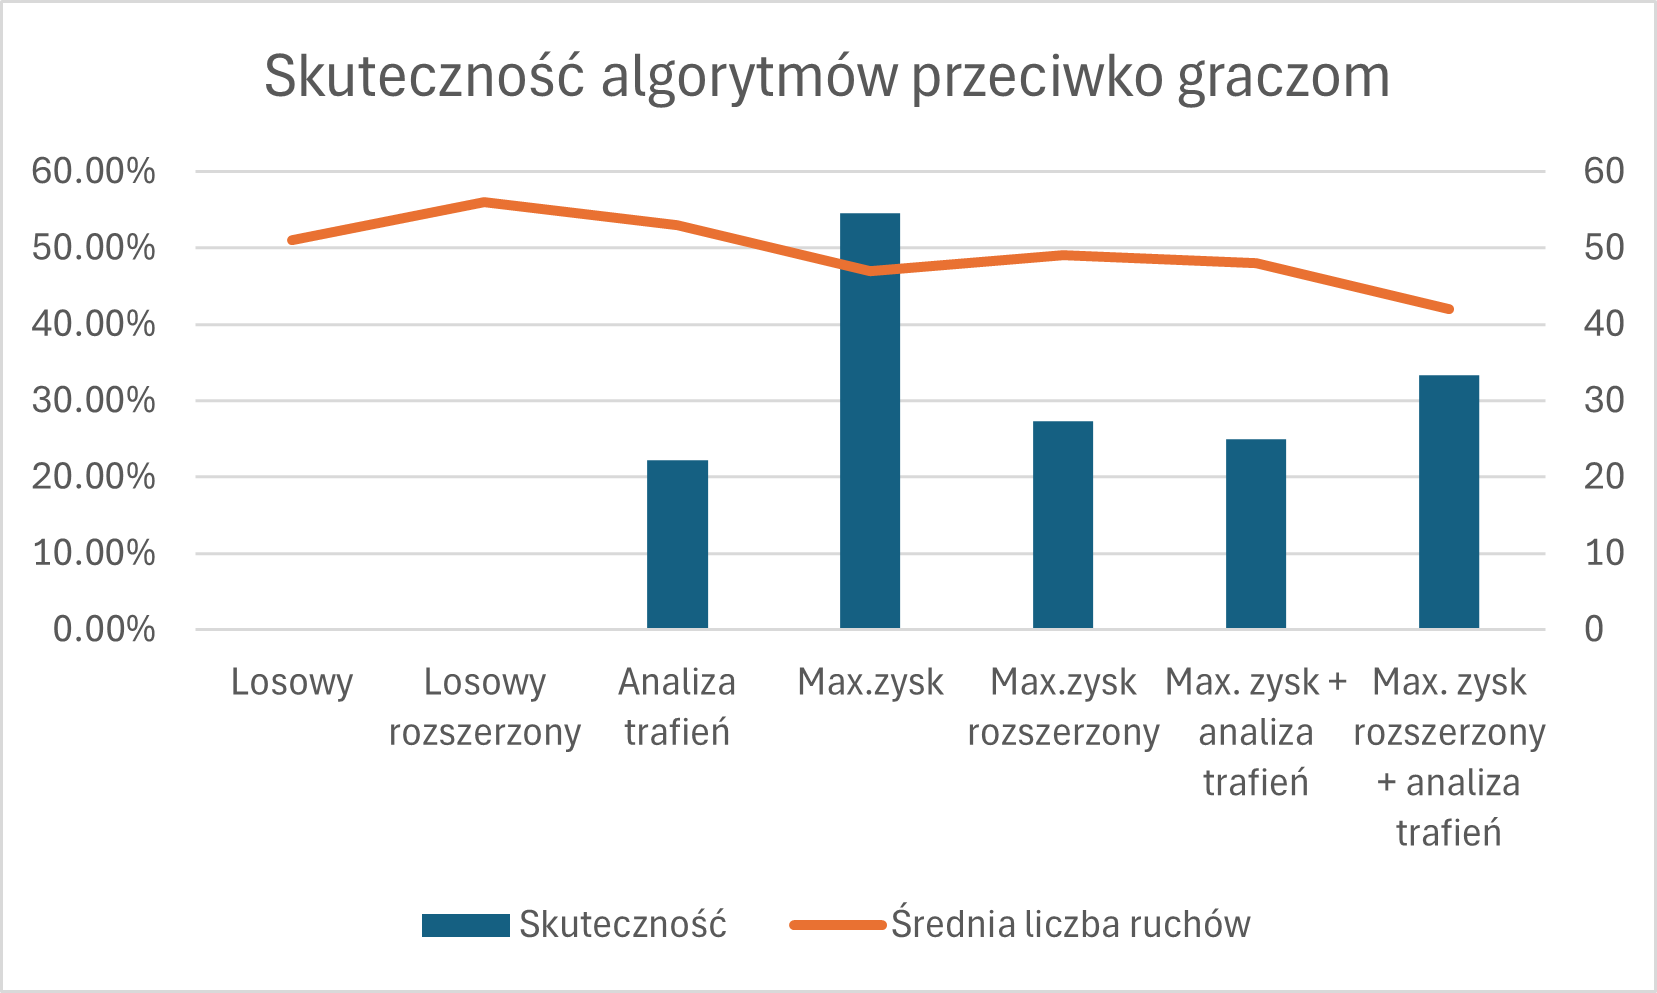
\includegraphics[width=0.9\linewidth]{img/vs_people_chart.png}
    \caption{Wykres przedstawiający skuteczność oraz średnią liczbę ruchów algorytmów w starciach z graczami.}
\end{table}